\documentclass[journal=jacsat, manuscript=article]{achemso}

\usepackage[version=3]{mhchem}
\usepackage[utf8]{inputenc}
\usepackage{natbib}
\usepackage{comment}
% \usepackage[dvipdfmx]{graphicx}
\usepackage{algorithm}
\usepackage[noend]{algpseudocode}
\usepackage{subcaption}

\newcommand{\argmax}{\mathop{\rm arg~max}\limits}
\renewcommand{\thesection}{\arabic{section}}

\title{Enhancing biomolecular sampling with reinforcement learning: a parallel tree search molecular dynamics simulation method}
% \title{Sampling protein folding conformations with parallel tree search selection molecular dynamics}
% \title{Tree search method for enhancing biomolecular sampling: an application in protein folding}

\author{Kento Shin}
\date{December 2018}

\begin{document}

\maketitle

\begin{abstract}
% PaCS MDに言及する必要なし.


% タンパク質の構造変化はその生物学的機能に大きく関わっており、分子動力学シミュレーション(MD)を用いて構造変化パスウェイを解明する試みが数多くなされている.
% Parallel Cascade Selection Molecular Dynamics (PaCS-MD)は短時間MDを繰り返し適用することで構造変化パスウェイを高速に探索する手法として提案されたが、局所安定構造に探索がトラップされてしまうという問題点を抱えている.本研究ではPaCS-MDを拡張し、UCTと呼ばれる木探索アルゴリズムを導入することで、Parallel Tree Search Molecular Dynamics (PaTS MD)という新たな手法を開発した.PaTS-MDはより広範囲を探索することが可能であり、局所構造から脱出しやすい手法である.実験によりChignolin, Trp-cageのフォールディングパスウェイ探索においてPaTS MDはPaCS MDよりも良い性能を達成した.


%Proteins conformation is crucially relevant to their biological functions. MD simulation has been widely used as a powerful tool to elucidate the proteins comformational transition mechanism. Parallel Cascade Selection Molecular Dynamics (PaCS-MD) is a method to search proteins comformational transition pathway quickly by performing short time MD simulation repeatedly. While PaCS-MD can successfully find the correct pathway in the simplest situation, it has a critical problem that it can be trapped in local optima since it works very "greedy". In this study, we extend PaCS-MD to a novel method, Parallel Tree Search Molecular Dynamics (PaTS-MD), by applying the tree search algorithm called UCT. PaTS-MD can search broader space and can escape from the local optima easier than PaCS-MD. PaTS-MD shows better performance than PaCS-MD in the experiment of searching the folding pathway of small proteins.

Proteins conformation is crucially relevant to their biological functions. Though molecular dynamics (MD) simulation has been widely used as a tool to sample protein conformations, the accessible time scale is not enough to observe the biological process. In this study, we developed a novel method, Parallel Tree Search Molecular Dynamics (PaTS-MD), to accelerate the search of conformational transition pathways. In PaTS-MD, a tree search algorithm is applied to choose a structure to perform MD simulation, which enable to avoid being trapped in a local stable structure and search broader space. PaTS-MD shows better performance than the existing method in the experiment of searching the folding pathways of small proteins, chignolin and Trp-cage.
\end{abstract}

\section{Introduction}
Proteins often undergo large-amplitude conformational transitions when they exert their biological functions such as protein-folding, enzyme catalysis, and molecular recognition with ligand binding proteins. Elucidating these structural transitions mechanisms is essential for understanding the biological functions. Since experimentally investigating the dynamics of protein conformational transitions is difficult, most of the knowledge from conformational transitions in proteins is derived from molecular simulation techniques.

Molecular Dynamics (MD) simulations is a powerful approach to find the pathway of protein conformational transitions. It can provide structural information as a time series of atomic-level trajectories with femtosecond time resolution. However, it is still be difficult to observe the large motion changes relevant to important biological functions because the accessible time scale of a conventional simulation is often too shorter than the characteristic time scales of the biological functions.
Furthermore, since conformational transitions relevant to biological functions occur stochastically, it is not ensured that the long-time MD simulations surely capture these rare conformational transitions.
To tackle this problem, many enhanced conformational sampling methods have been proposed  

Parallel Cascade Selection Molecular Dynamics(PaCS-MD) \citep{harada2013parallel} is one of the methods to find the conformational transition pathway between initial structure and target structure when both structures are known {\it a priori}. In PaCS-MD, multiple short-time MD simulations are simply repeated until it reaches the structure sufficiently closer to the target structure.
Though PaCS-MD can fast generate the transition pathway to the target structure without adding any force bias, it has a critical problem that it can be trapped in stable local optima since PaCS-MD is a quite greedy algorithm. In other words, once PaCS-MD reaches a stable local free-energy minima, it cannot escape from it and search another way.

To solve this problem, in this study, we extend PaCS-Md by applying a tree search algorithm called UCT \citep{kocsis2006bandit} and propose a new method, Parallel Tree Search Molecular Dynamics (PaTS-MD). UCT is a tree search algorithm in which it select the node by balancing the trade-off between searching a node with best score and one which is not best now but is likely to become best if search more.
UCT can avoid being trapped in a stable local optima because nodes which are visited many times are penalized and are unlikely to be selected again. Therefore PaTS-MD can escape from a local minima even if it is trapped, and  can search broader space than PaCS-MD.

In the experiment, we compared PaCS-MD and PaTS-MD by applying both methods to folding study of mini-protein, chignolin and Trp-cage. In both experiment, we confirmed that PaTS-MD had more possibility to find the correct pathway.

\section{Method}
\subsection{Procedure of PaCS-MD}
Figure \ref{fig:pacs_and_pats_mehtod}(a) shows a brief illustration of PaCS-MD method. In PaCS-MD, both "reactant" and "product" structures are given {\it a priori}. PaCS-MD starts from the initial structure (reactant) and continues until it reaches the structure sufficiently close to the target structure (product) by repeating short Multiple Independent Molecular Dynamics (MIMD) simulations. In each cycle of PaCS-MD, M short MIMD starting from different snapshot were performed by giving different initial velocity randomly to each initial structure. Then generated snapshots are rank-ordered with respect to the similarity to the product structure. Root-mean-square-deviation from the product structure is employed to measure the similarity to the product structure. Top M snapshots are selected as the initial structures  for the next cycle. This cycle is subsequently repeated until highly ranked snapshots reach the sufficiently close to the product. After that, we can generate a trajectory from the reactant to the target by connecting all trajectories in each cycle. 

Since PaCS-MD is a pretty "greedy" algorithm, which means that it always chose the way which looks best based on the knowledge obtained so far, it can be trapped in a local stable minimum structure. 



\subsection{Procedure of PaTS-MD}

\begin{figure}[t]
\centering

\includegraphics[width=15cm]{Figures/pacs_and_pats_method.png}
\caption{A procedure of (a) PaCS-MD, (b) PaTS-MD } 
\label{fig:pacs_and_pats_mehtod}
6\end{figure}

PaTS-MD is a novel extension of PaCS-MD by applying tree search method to avoid being trapped in local optima. In the tree search, tree is composed of node and edge and gradually constructed as the search goes on. In PaTS-MD, the node is the protein structure and the edge is the trajectory between two structures obtained by the short MD simulations. 

We applied UCT algorithm in PaTS-MD. UCT is a kind of Monte Carlo Tree Search algorithm which is successful mainly in computer GO problem. UCT treat the choice of child node as a multi-armed bandit problem. UCT can address the exploration-exploitation dilemma of bandit problem by choosing the child nodes which has the maximum Upper Confidence Bound (UCB). UCB of i'th child node is represented as follows.
\begin{equation}
UCB_{i} = X_i + C \sqrt{\frac{2\log{N}}{n_i}},
\end{equation}
where $N$ is the number of times the parent node has been visited, $n_j$ is the number of times child j has been visited, $X_i$ is a value of the node i and $C$ is a constant to balance exploration and exploitation. We use a negative of minimum RMSD of the downstream nodes as $X$. The reason why negative RMSD is used is that we want to minimize the RMSD although UCT is basically designed to find the maximum. UCB deal with the trade-off between  the first (exploitation) and second (exploration) terms. At first, a node with high $X$ is likely  to be selected. But as the number of times $n$ increases, UCB gradually decrease and another child node become likely to be selected. Thanks to this property, PaTS-MD can escape from the local stable optima. Obviously, how much it tends to do exploitation or exploration is strongly dependent on value of constant $C$.
The appropriate value of $C$ is determined by the complexity of the target system and the length of available time.
One cycle of PaTS-MD consists of selection, expansion, backpropagation steps as shown in Figure \ref{fig:pacs_and_pats_mehtod}(b).
In the selection step, the tree is traversed from the root to a leaf by choosing the child with maximum UCB recursively at each branch. If more than one child node have the same maximal value, the one of which is chosen randomly. In the expansion step, short MD simulation is performed from the selected node and the snapshot with minimum RMSD is added as a child of the selected node. If RMSD does not decrease, it is not added. Finally, in the backpropagation step, the visit count of each ancestor node is incremented by one and value $X$ is also updated if obtained RMSD is less than the original one. The detail process of these steps are illustrated as pseudocode in Algorithm \ref{alg:pats}.

\subsection{PaTS-MD with penalization}
To avoid being trapped to local stable structure more, we penalize the value $X$ based on how many similar structures are already searched.
The penalized value $X'$ is calculated as follows.
\begin{equation}
X'_i = X_i * \alpha^{N\_similar}, 
\end{equation}
where $\alpha$ is the penalty constant and N\_similar is the number of similar structure to i'th structure. The similar structure is defined as the structure whose RMSD to i'th structure is less than 0.5 \AA.
This penalization prevent to search the states with high frequency area and encourage to search the states with low frequencies. Moreover, it transmits the information from one branch to other branches, which can reduce the number of searches which are already done by another branch.

\subsection{Computational Details}
% Calculation performed in this study (parameters of PaCS-MD, PaTS-MD, snapshot sampling frequencies etc…, simulation parameter used: thermostat, barostat, timestep etc, equilibrating methods before production simulations…

To demonstrate the performance of PaTS-MD, we applied both PaCS-MD and PaTS-MD methods to folding small proteins, chignolin and Trp-cage in the explicit water.

NMR structure (PDB ID: 2RVD for chignolin, 1L2Y for Trp-cage) are used as a target, and artificially extended structure as a reactant.
ABMER ff99SB force field was employed for both systems. The simulated systems were solvated with SPC/E water model for chignolin and TIP3P water model for Trp-cage. Rectangular simulation boxes were constructed with a margin of at least 10  \AA \  from the proteins to the box boundaries.
The chignolin system contained 5712 water molecules and 2 NA$^+$ ions. The Trp-cage system contained 18980 water molecules and 1 Cl$^-$ ion.

In each cycle of PaCS-MD and PaTS-MD, 100-ps MD simulation was performed under constant temperature condition at 300K for chignolin and 320K for Trp-cage using V-rescale thermostat. The electorostatic interactions were treated with particle mesh Ewald method. The simulation time step was 2 fs with constraining all bonds via LINCS and snapshots in each trajectory was recorded every 1ps. All the MD simulations were performed with the GPU version of the GROMACS 2016.5 package. 

In the demonstrations, PaCS-MD and PaTS-MD cycle was repeated until C$_\alpha$ RMSD to the native structure was less than 1.0 \AA. We set the number of parallel cascades in PaCS-MD as 5 and the maximum number of children nodes in PaTS-MD as 3.


% \begin{comment}
\begin{algorithm}[ht]
\caption{PaTS-MD algorithm}\label{alg:pats}
\begin{algorithmic}[0]
\Function{PaTS-MD}{}
\State create $rootnode$
\State $node \gets node_0$
\While{$node.X > RMSD\_MIN$}
\State $node \gets$ \Call{Select}{$rootnode$}
\State $child \gets$\Call{MakeChild}{node}
\State $X \gets$\Call{MDrun}{$child$}
\If{$X < node.X$}
\State \Call{AddChild}{$child, node$}
\EndIf
\While{$child \not= rootnode$}
\State $Backpropagete(child, -X)$
\State $child \gets child.parent$
\EndWhile
\EndWhile
\EndFunction
\\
\Function{MakeChild}{$parent$} \label{func:makechild}
\State $node \gets object$
\State $node.v \gets 0$
\State $node.X \gets \infty$
\State $node.X_{max} \gets \infty$
\State $node.parent \gets parent$
\State \Return $node$
\EndFunction
\\
\Function{AddChild}{$node, parent$} \label{func:addchild}
\State $parent.children \gets [parent.children, node]$
\EndFunction
\\
\Function{Select}{$node$} \label{func:select}
\While{$length(node.children) < MAX\_CHILDREN$}
\State $node \gets \argmax_{v' \in children \: of \: v} node.X_{max} + C \sqrt{\frac{2\log(node.parent.v}{node.v})}$
\EndWhile
\State \Return{$node$}
\EndFunction
\\
\Function{MDrun}{$node$} \label{func:mdrun}
\State $traj \gets$ MDsimulate from the $node.parent.structure$
\State $node.structure \gets$ choose the snapshot with minimum RMSD in the $traj$
\State $node.X \gets$ minimum RMSD in the $traj$
\State \Return{node.X}
\EndFunction
\\
\Function{Update}{$node, X$} \label{func:update}
\State $node.v \gets node.v + 1$
\If{$X > node.X_{max}$}
\State $node.X_{max} \gets X$
\EndIf
\EndFunction
\end{algorithmic}
\end{algorithm}
% \end{comment}



\section{Result}
% RMSD plot, Bar plot
% Tree graph colored by order, native contact, hydrogen bond
% structure figure
% Projection on free energy landscape

\begin{figure}[ht]
\begin{minipage}[b]{0.49\textwidth}
\centering
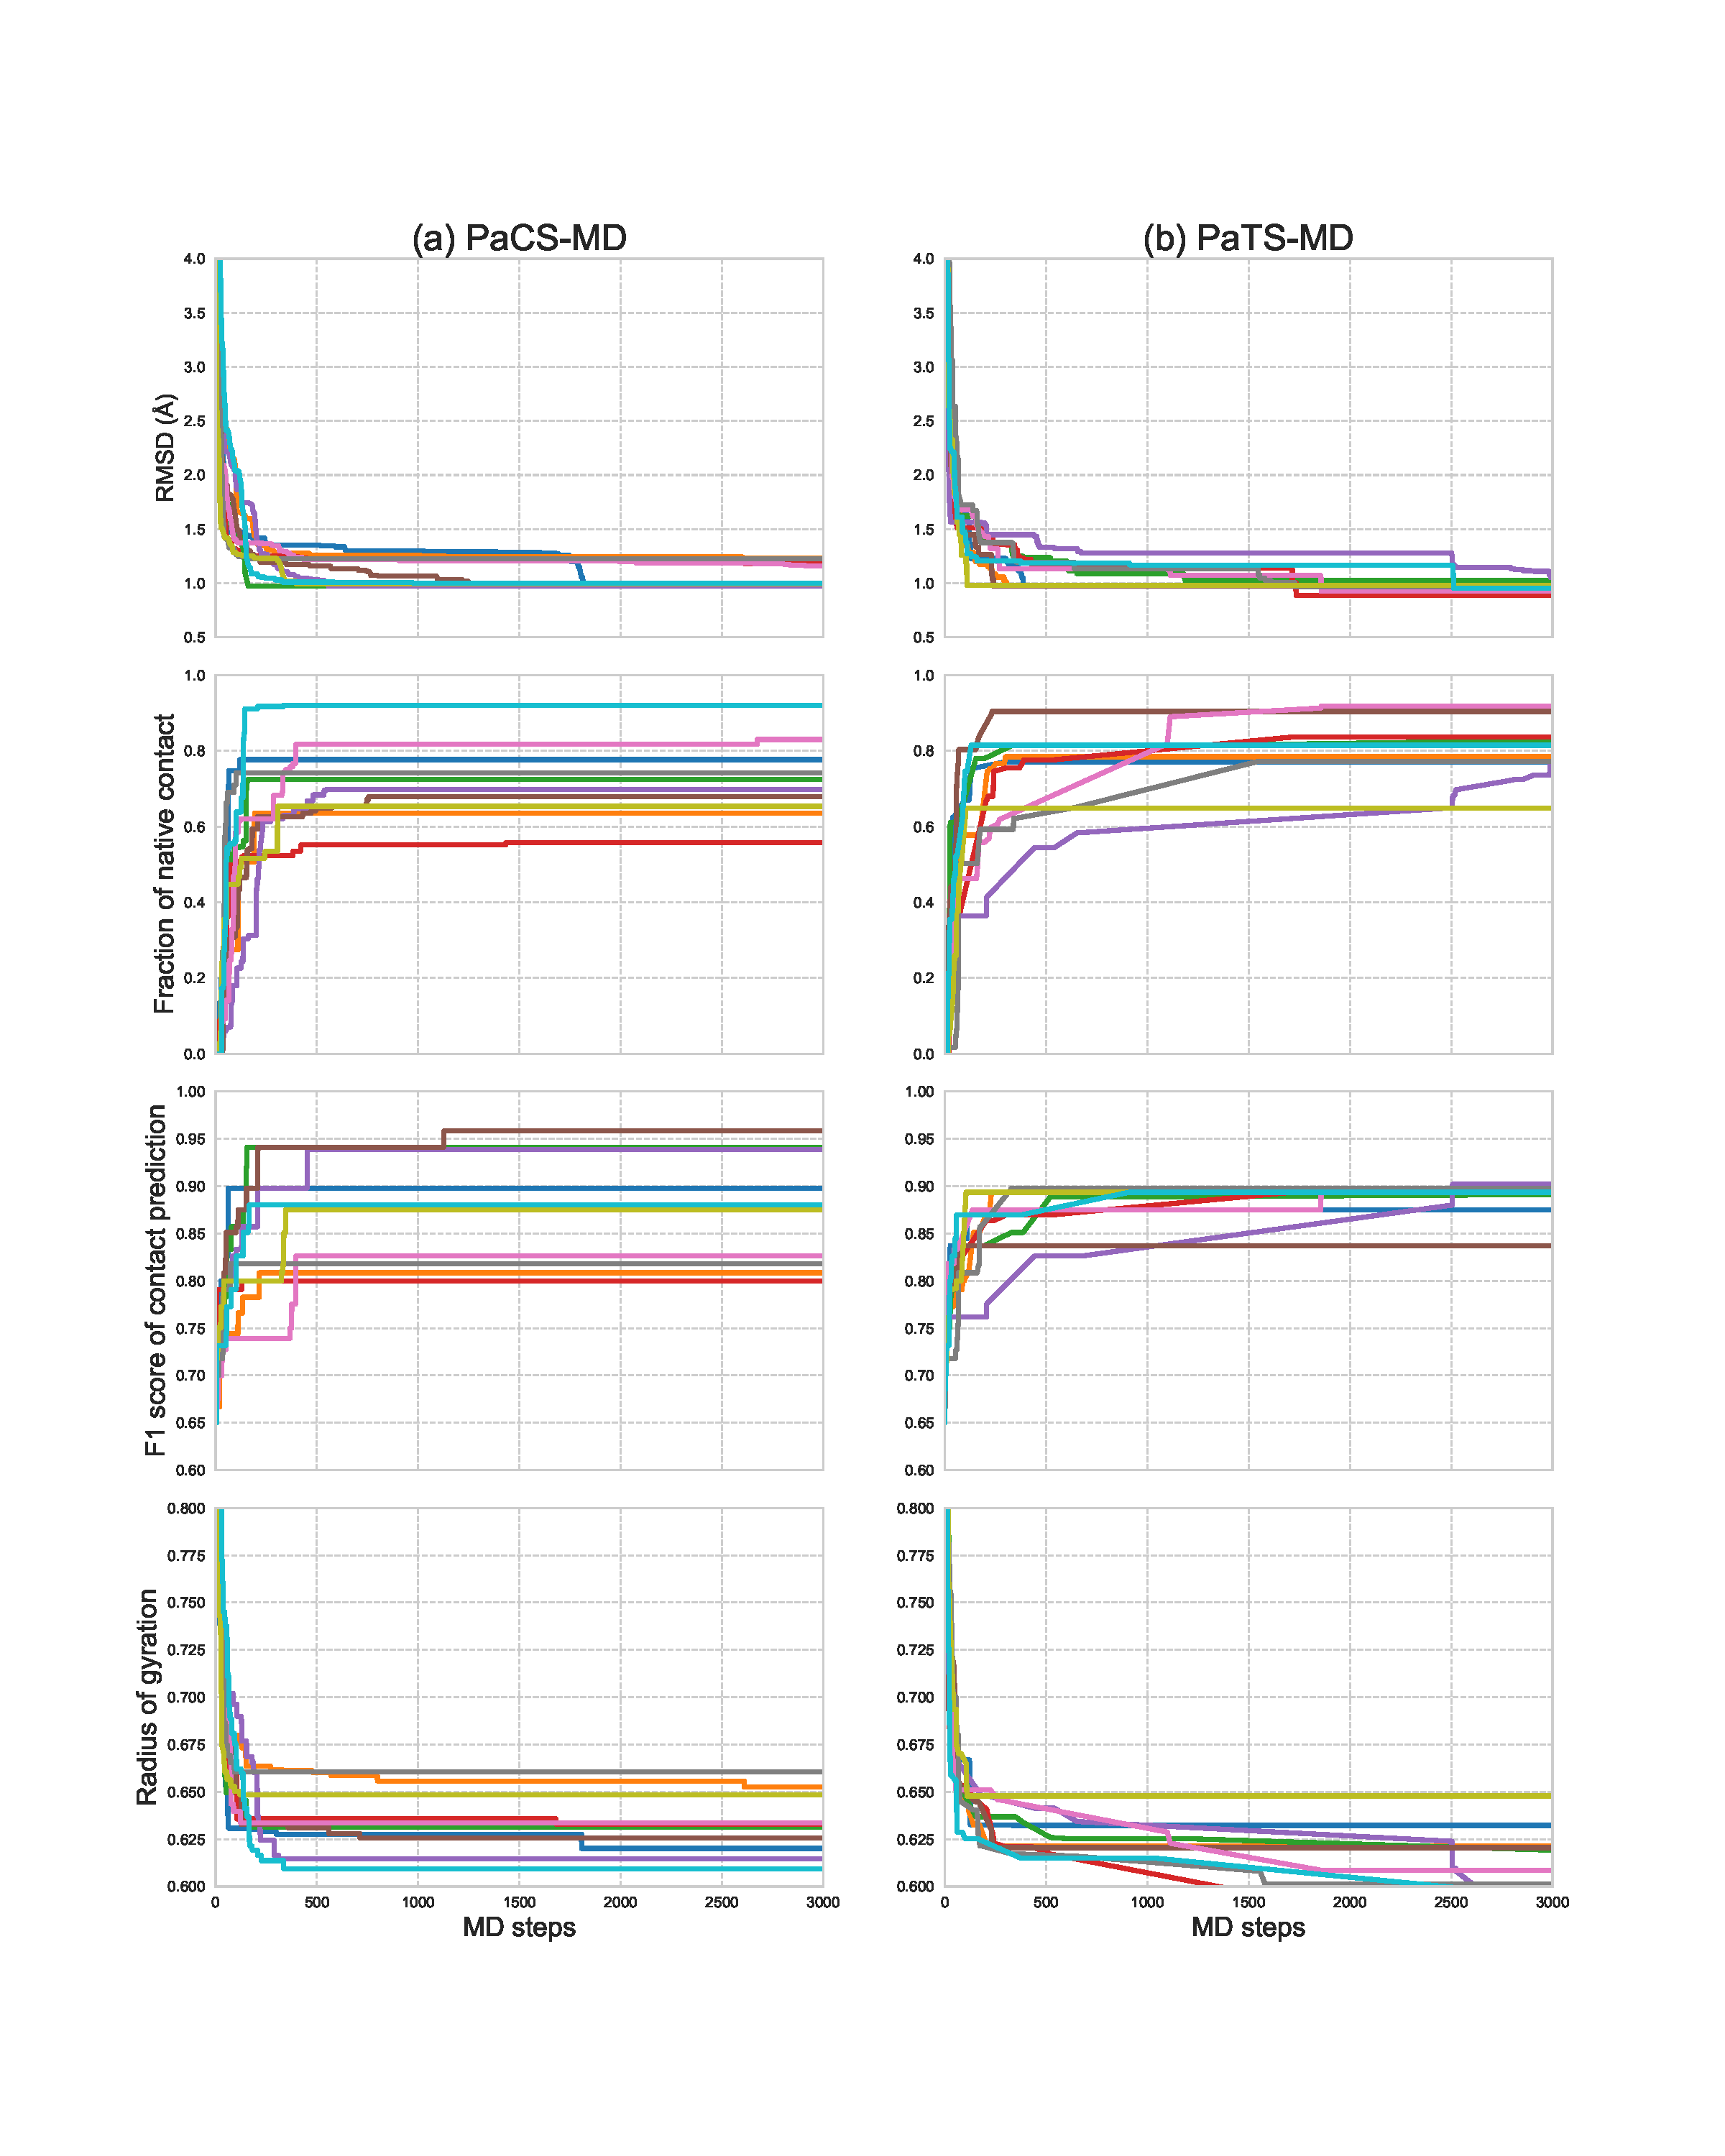
\includegraphics[width=1.0\textwidth]{Figures/chig_plot_both.pdf}
\caption{PaCS}
\label{fig:result_pacs_plot}
\end{minipage}
\begin{minipage}[b]{0.49\textwidth}
\centering
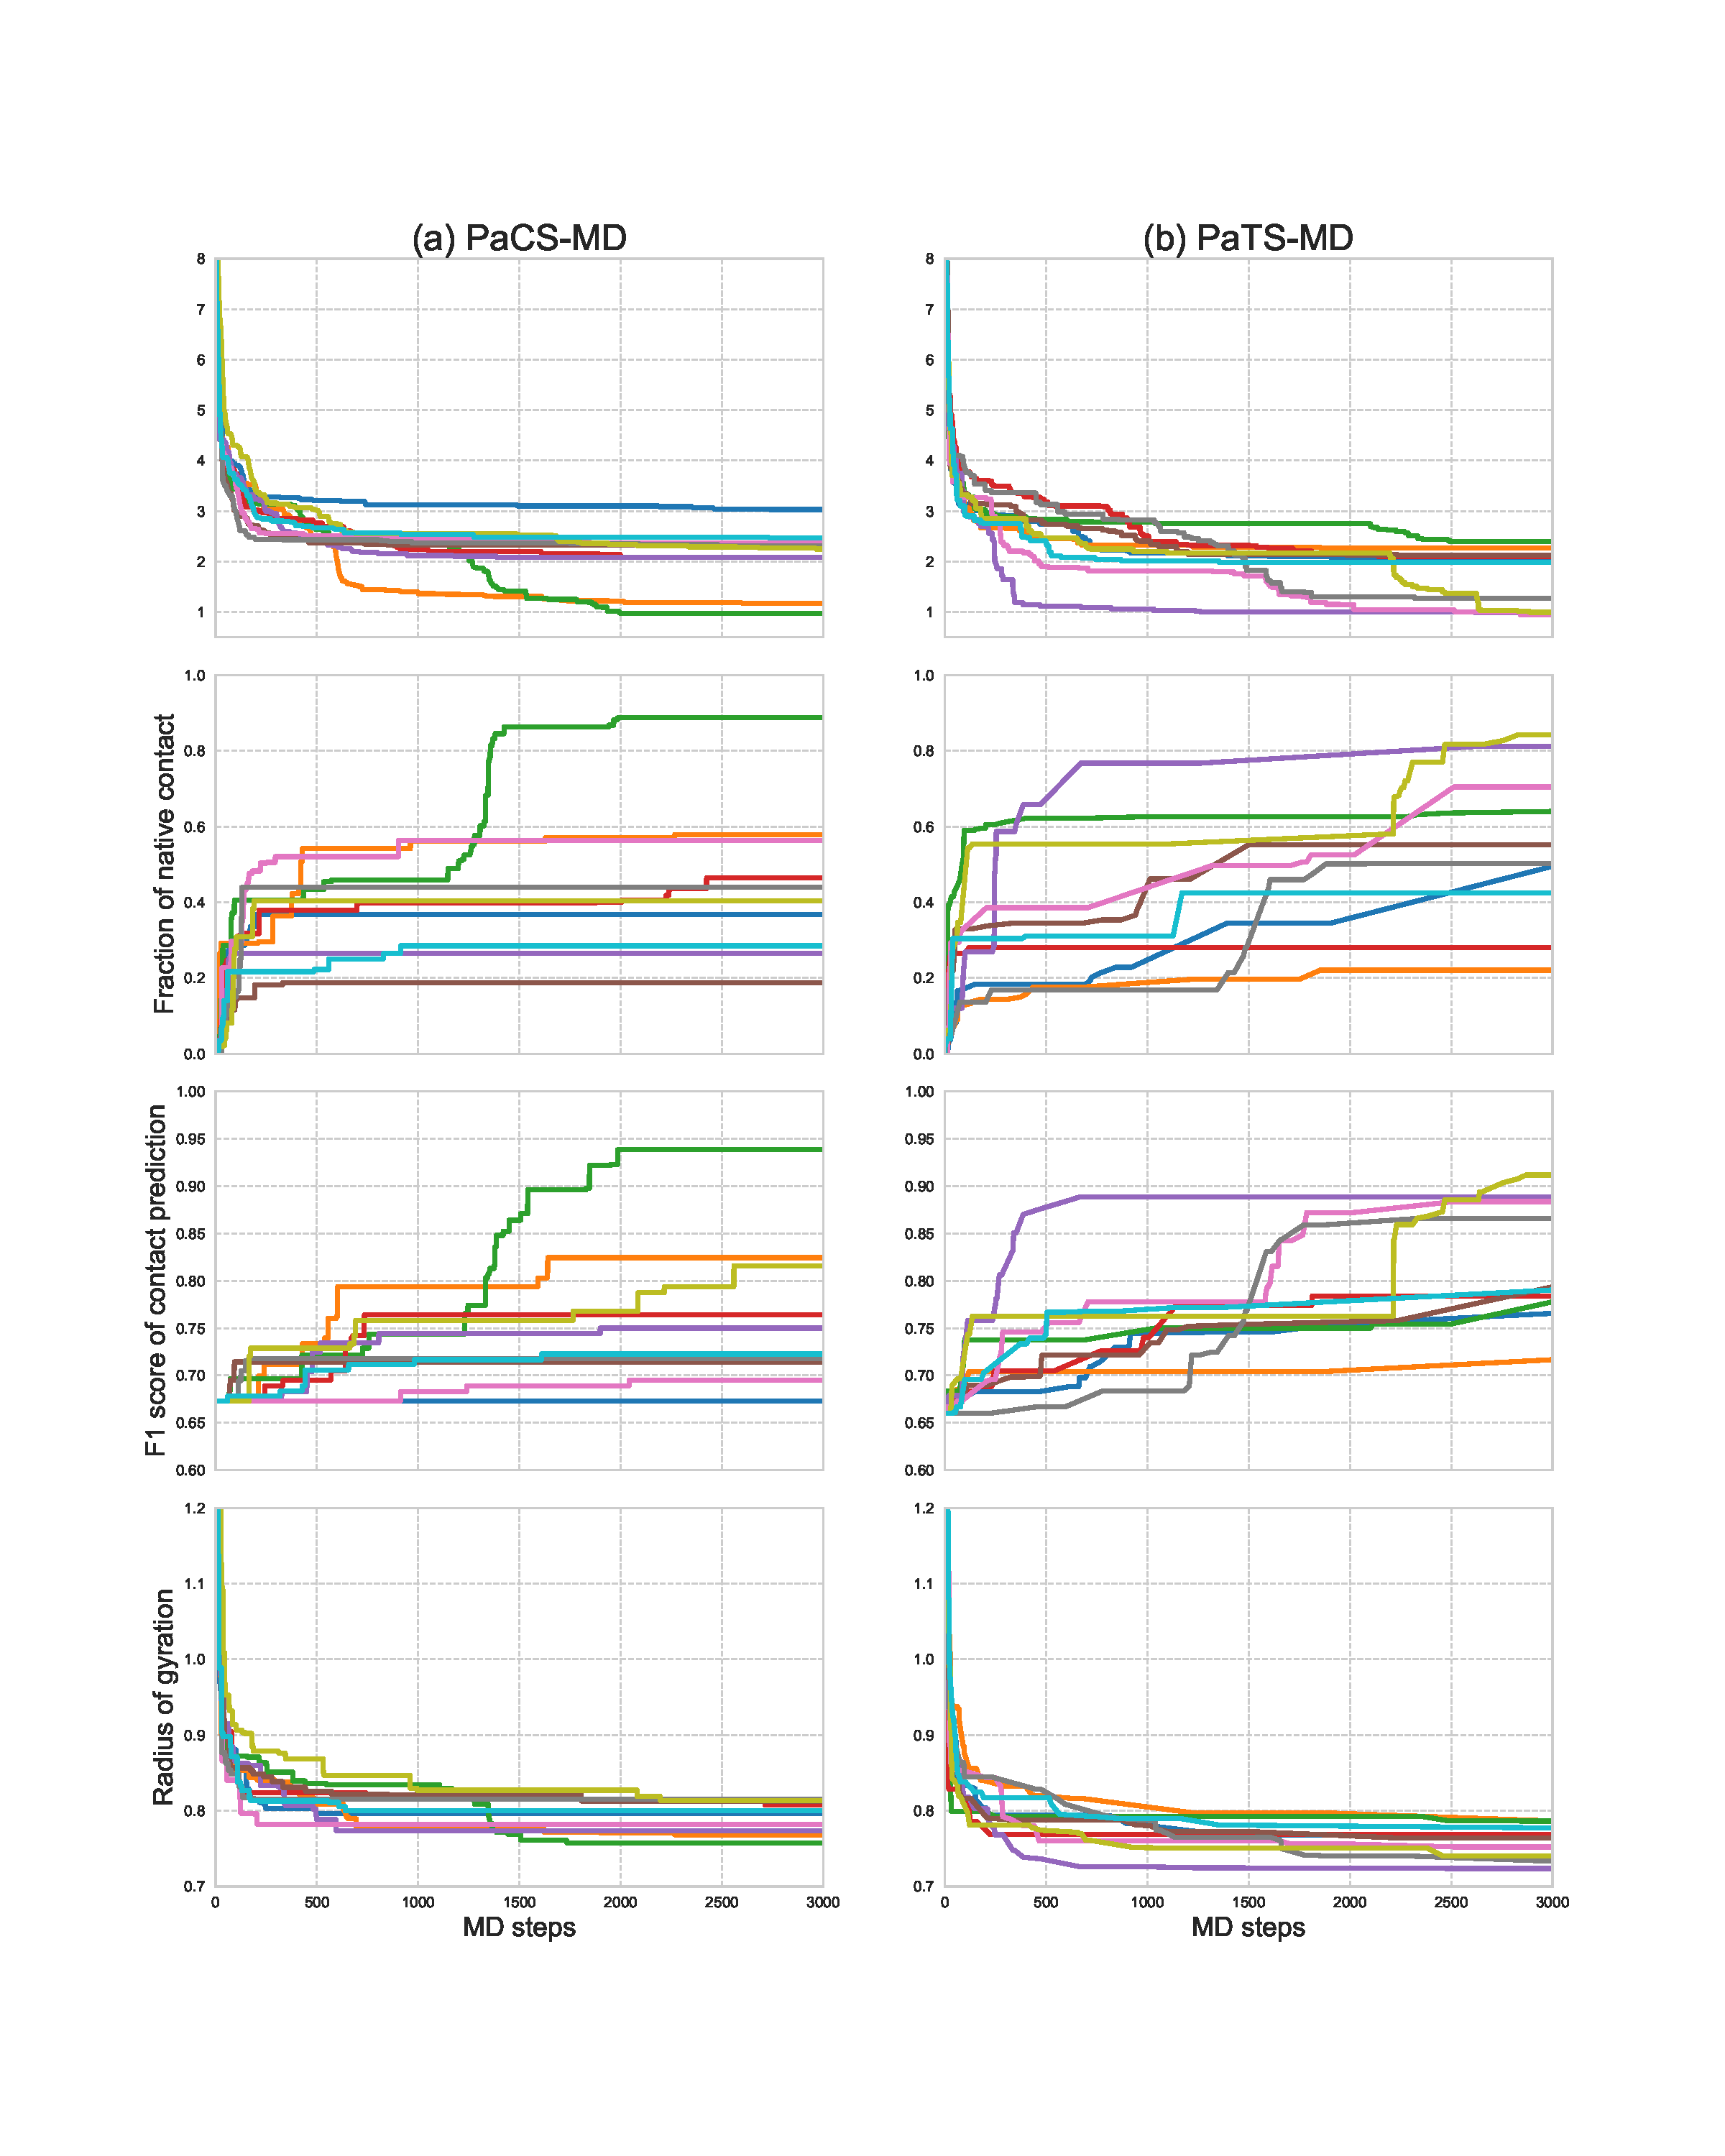
\includegraphics[width=1.0\textwidth]{Figures/trp_plot_both.pdf}
\caption{PaTS}
\label{fig:result_pats_plot}
\end{minipage}
\end{figure}

\begin{figure}[ht]
\begin{minipage}[b]{0.95\textwidth}
\centering
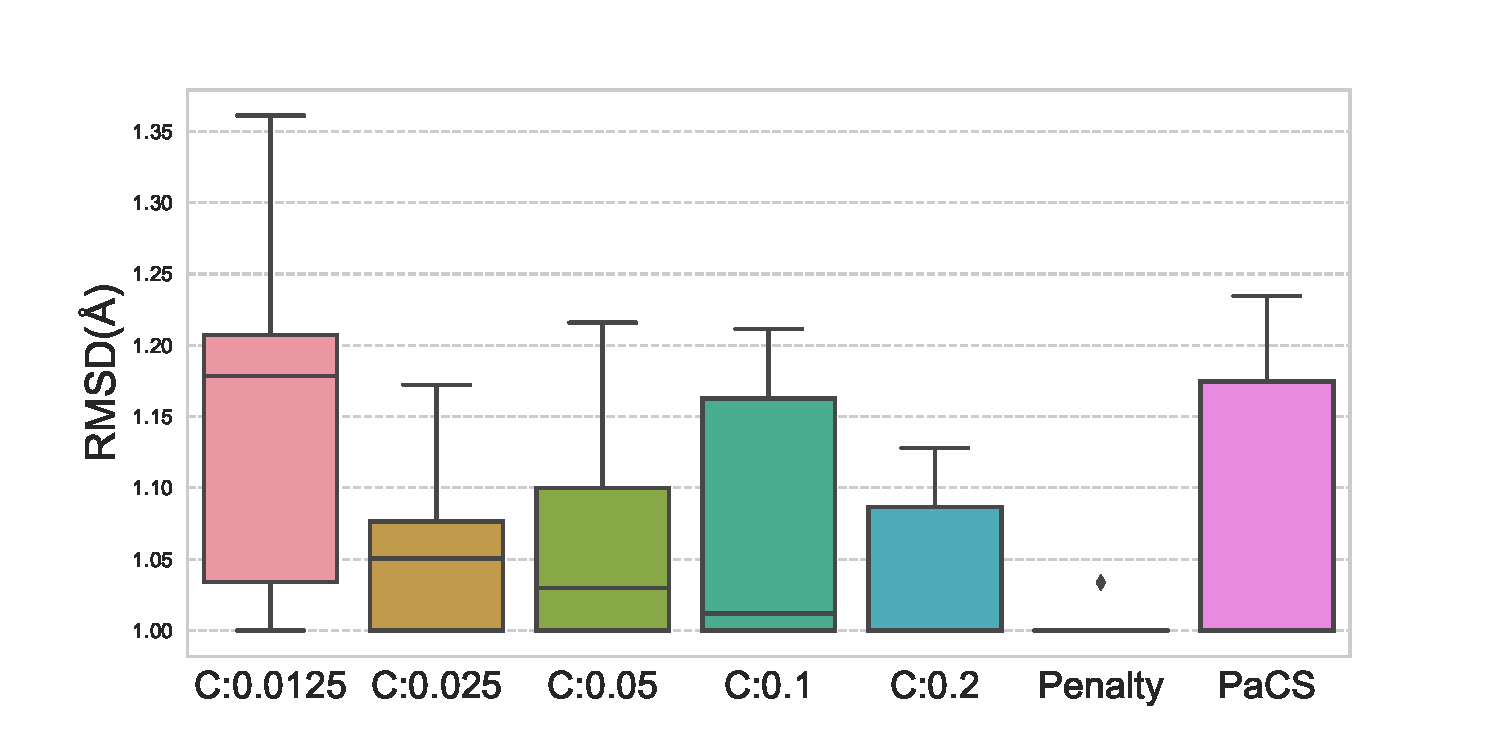
\includegraphics[width=0.9\textwidth]{Figures/chignolin_result_boxplot.pdf}
\subcaption{Chignolin}
\end{minipage}
\begin{minipage}[b]{0.95\textwidth}
\centering
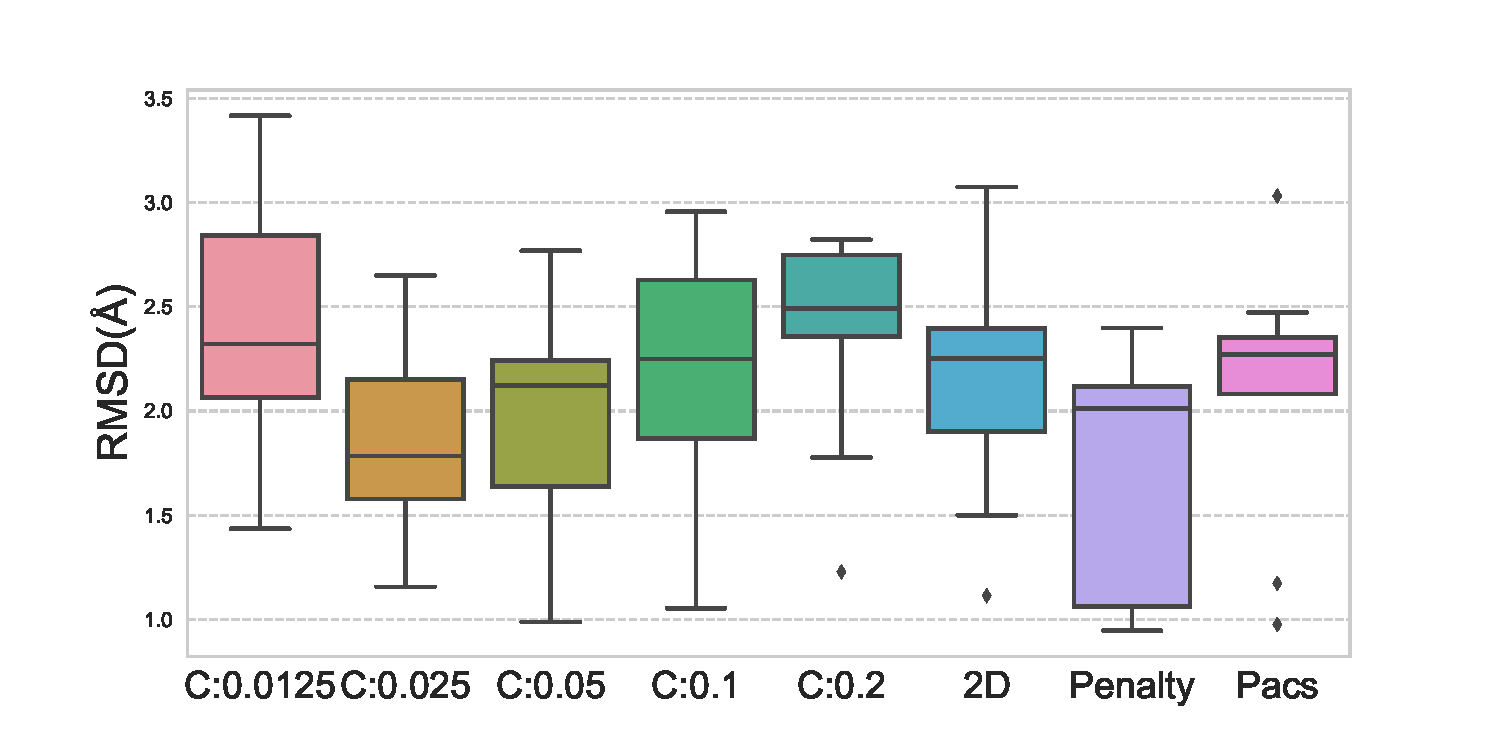
\includegraphics[width=0.9\textwidth]{Figures/trpcage_result_boxplot.pdf}
\subcaption{Trp-cage}
\end{minipage}
\caption{Boxplot}
\label{fig:result_box}
\end{figure}


\subsection{Chignolin Folding}
To search the reactive trajectories of folding pathway of Chignolin in explicit solvent, PaCS-MD and PaTS-MD were performed up to 3000 MD steps. In PaTS-MD, $C$ was set to 0.05 and penalization parameter $\alpha$ was set to 1.05. 

Figure \ref{fig:result_pacs_plot} shows various profiles of 10 trials of PaCS-MD and PaTS-MD as a function of MD steps, which includes RMSD, fraction of native contact, f1 score of contact prediction and radius of gyration. (An explanation of fraction and f1). 
This profiles shows that the protein gradually changes its structure to the product as MD simulation goes on.
In both PaTS-MD and PaCS-MD, some trials can reach the product but others stopped at around 1.2 \AA. It implies that there is a local stable optima around the native structure.
To demonstrate penalization works to make search efficient, PaTS-MD without penalization with different $C$ were also performed.

Figure \ref{fig:result_box}(a) shows a boxplot of RMSD at 3000th steps to summarize the performance of each method. 6 trials successfully reached the product in PaCS-MD and 8 trials in PaTS-MD. In PaTS-MD without penalization, the different $C$ resulted in different performance. It indicates that the choice of C affect the exploration and exploitation trade-off, the smaller $C$ is more likely to explore and larger $C$ is more likely to exploit. The performance of PaTS-MD with penalization is better than PaTS-MD without penalization with any $C$. This result prove that penalization allows search more efficient.
Figure \ref{fig:tree_chig} shows the search tree of each methods with some structures correspond to each node. The tree is colored along the order when each node is added to the tree.
In PaCS-MD, tree goes on deeply and does not search broad area. Though it sometimes can find the correct pathway very fast, it is also possible to be trapped to a local optima. In contrast, PaTS-MD can searches many branches in one tree. Then it can "escape" from the local optima even once it reaches as shown in Figure \ref{fig:tree_chig}(b)(c).

\subsection{Trp-cage Folding}
To search the reactive trajectories of folding pathway of Trp-cage in explicit solvent, PaCS-MD and PaTS-MD were performed up to 3000 MD steps. In the PaTS-MD with penalization, $C$ was set to 0.05 and $\alpha$ as 1.01.

Figure \ref{fig:result_pacs_plot} shows the profiles of 10 trials of PaCS-MD and PaTS-MD with. Searching the reactive trajectory of Trp-cage folding is more difficult than Chignolin folding because the size of Trp-cage is larger and more complicated. Only 1 trial successfully reached the product in PaCS-MD, 3 trials reached in PaTS-MD. Although PaCS-MD is likely to become "flat" after some point, PaTS-MD could improve the profiles as MD steps went on. It indicates that PaTS-MD tries to search other better branches after it reaches the local stable structure. 
Figure \ref{fig:result_box}(b) shows a boxplot of RMSD at 3000th steps of each method. Clearly, the PaTS-MD with penalization results better performance than PaCS-MD. 

Figure \ref{fig:tree_trp} shows the search tree of each methods. It can be seen that PaTS-MD searched broader spaces than PaCS-MD. As shown in Figure \ref{fig:tree_trp}(b)(c), it reaches the misfolded structure whose alpha helix is wrong at first then it start to search other branches and found the correct pathway after all. 

To examine the detail behavor of sampling, trajectories were projected onto a sub-space spanned by .....
% Free energy landscape

\begin{figure}[t]
\centering
 \begin{minipage}{0.3\hsize}
 \centering
 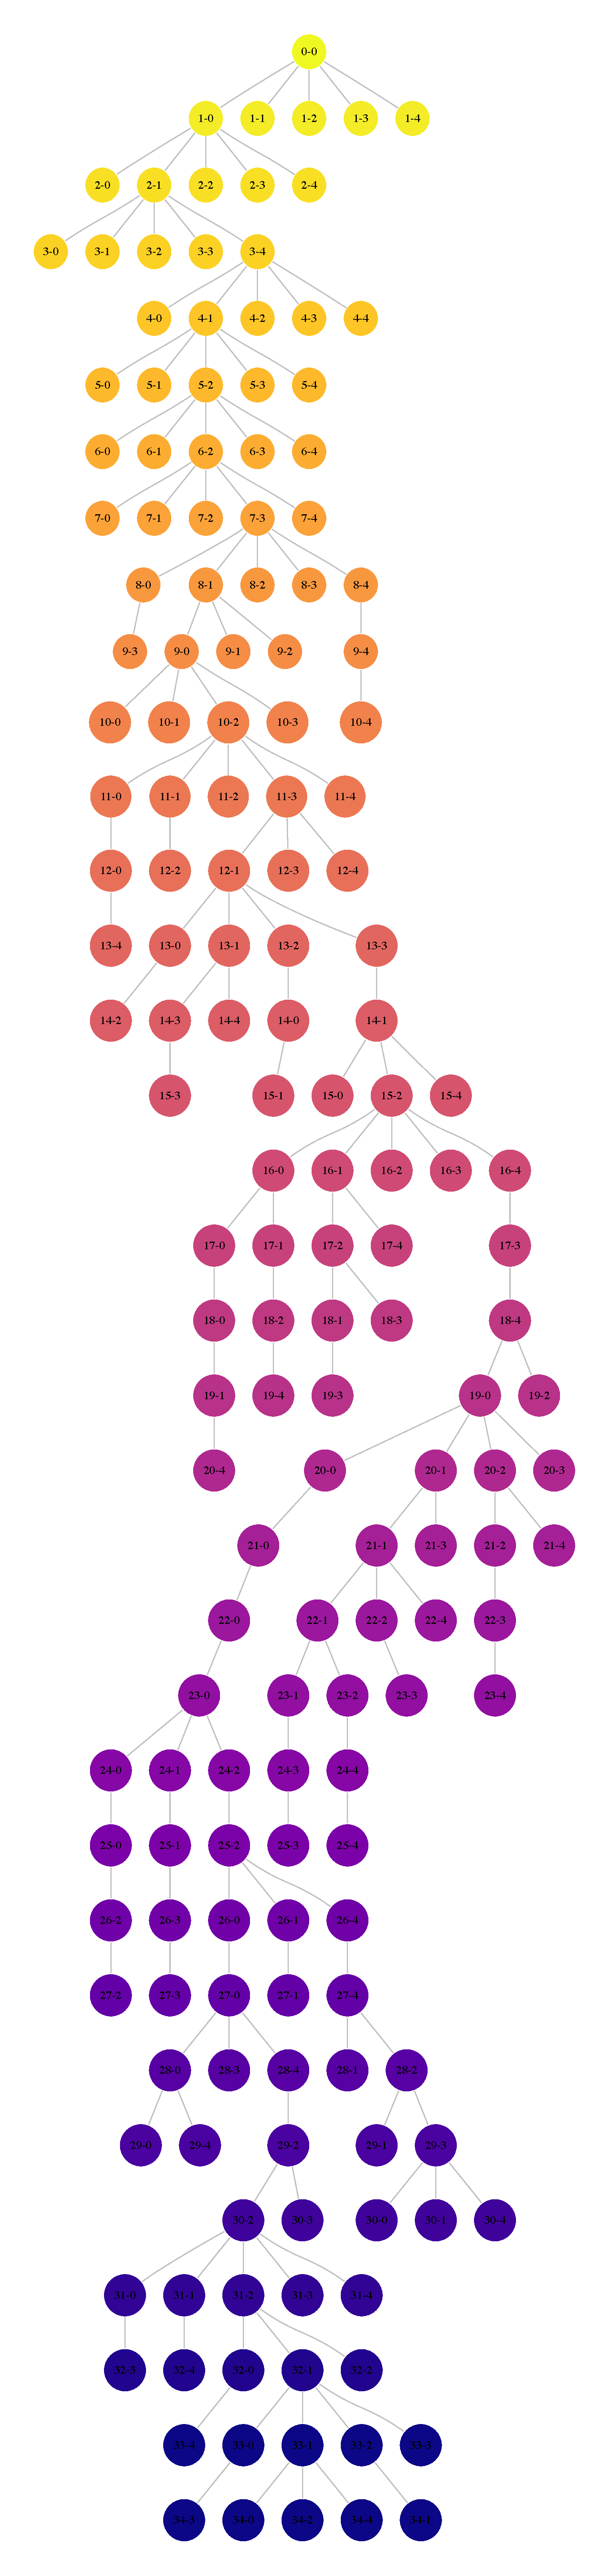
\includegraphics[scale=0.08]{Figures/tree_chi_pacs_best.pdf}
 \subcaption{PaCS}
 \end{minipage}
 \begin{minipage}{0.6\hsize}
 \centering
 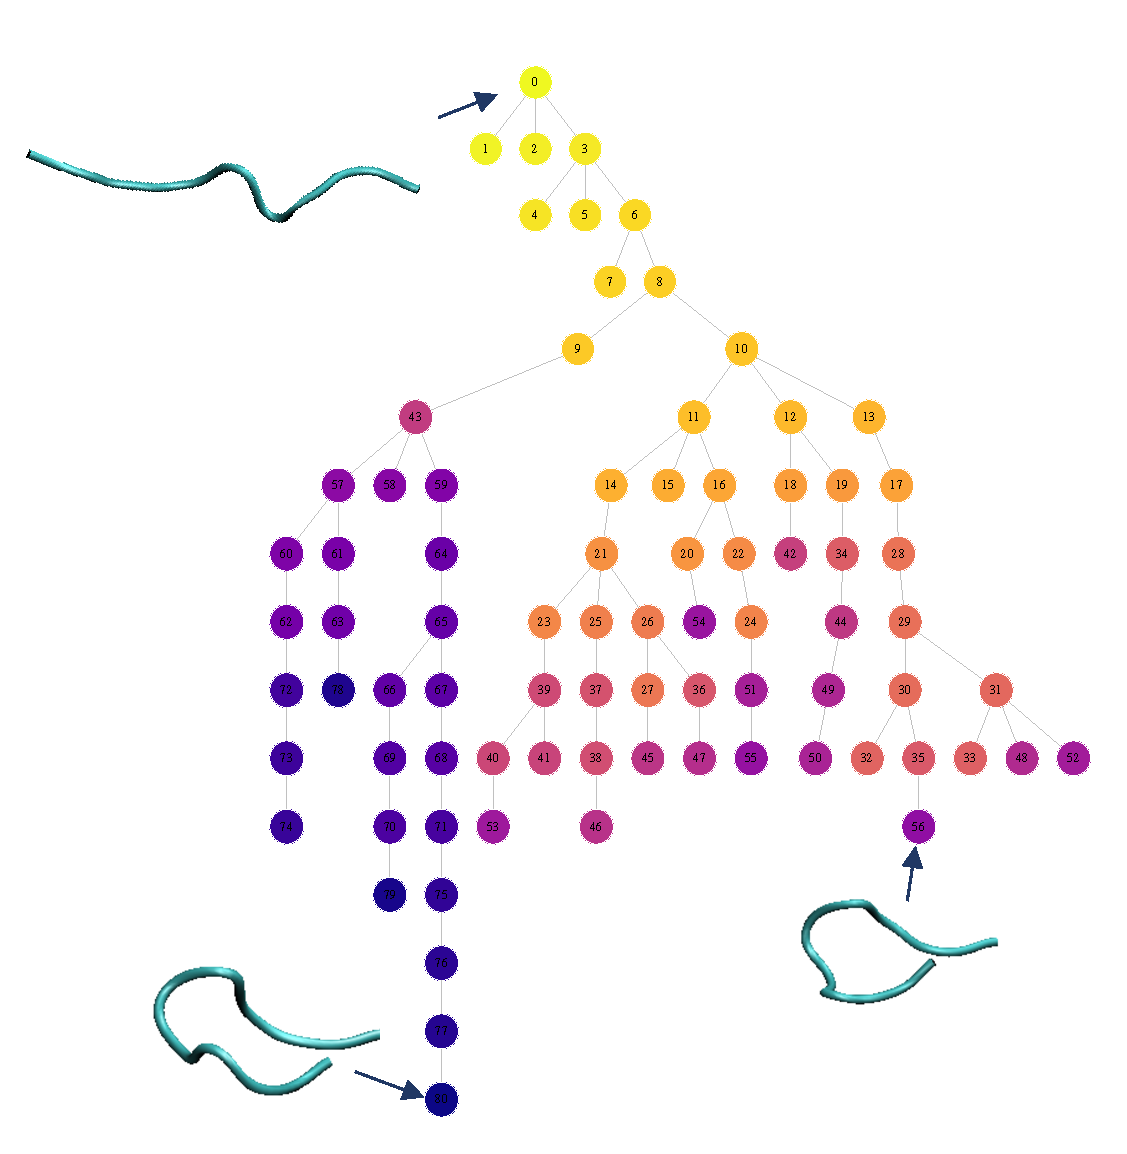
\includegraphics[scale=0.3]{Figures/tree_chi_pats.pdf}
 \subcaption{PaTS}
 \end{minipage}
\begin{minipage}{0.95\hsize}
\centering
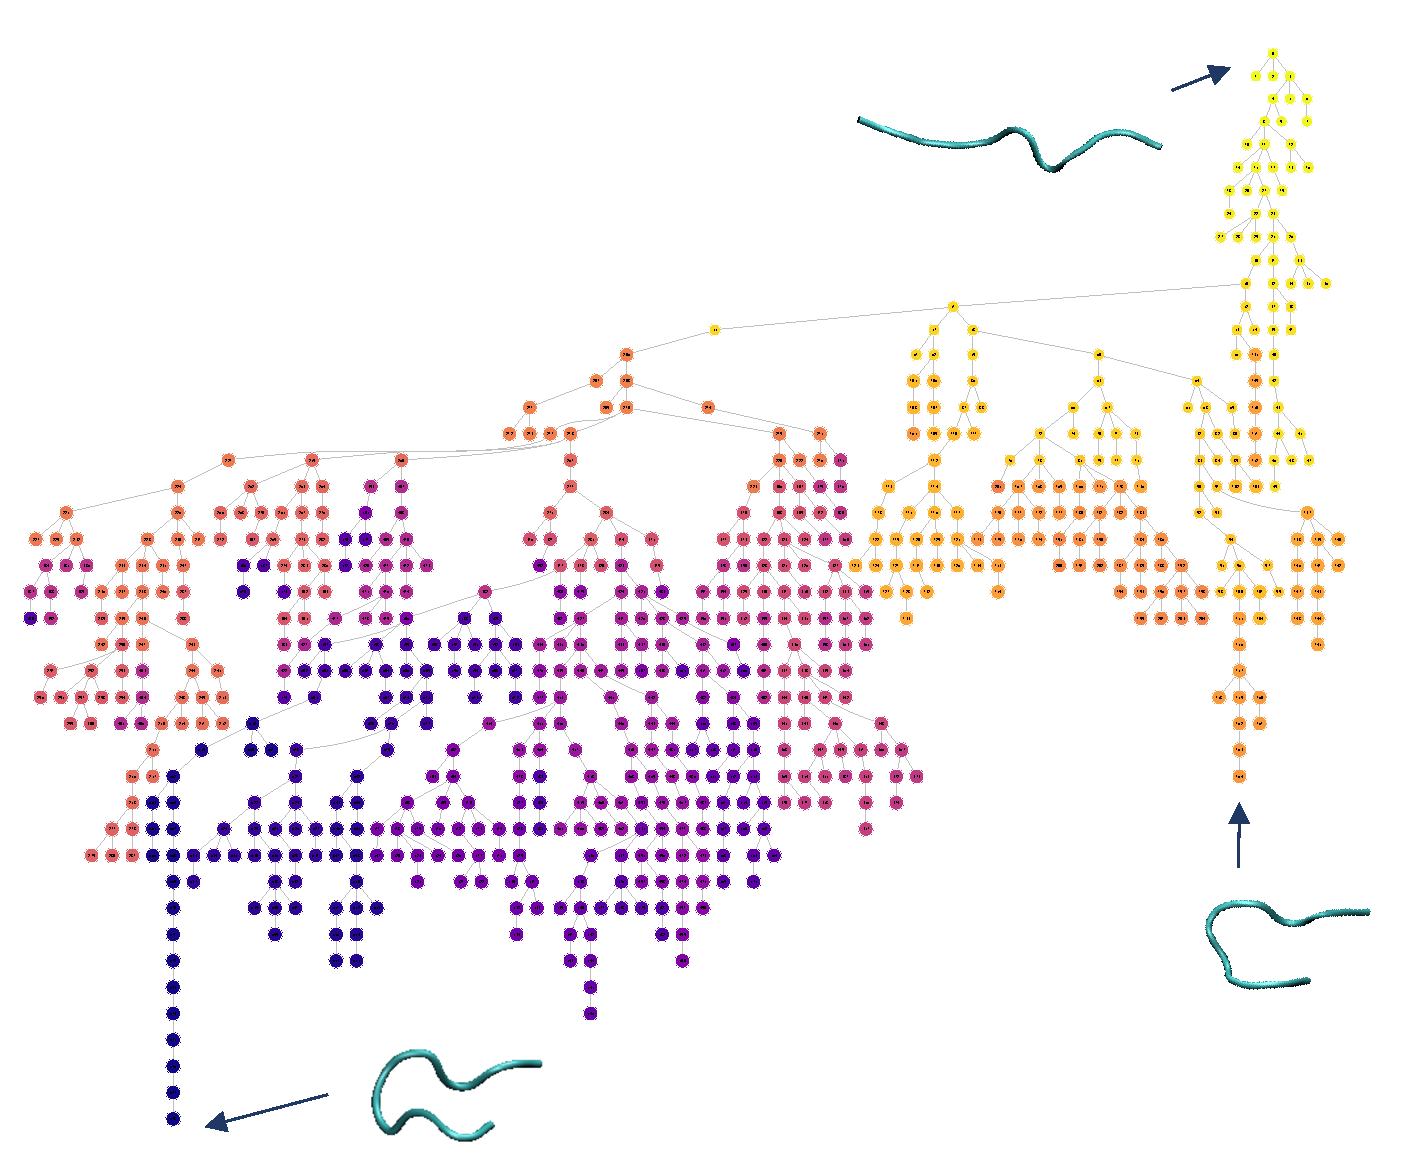
\includegraphics[scale=0.5]{Figures/tree_chi_pats_penal.pdf}
\subcaption{PaTS penalization}
\end{minipage}
\caption{Trees of Chignolin folding in each methods}
\label{fig:tree_chig}
\end{figure}

\begin{figure}[t]
\centering
 \begin{minipage}{1.0\hsize}
 \centering
 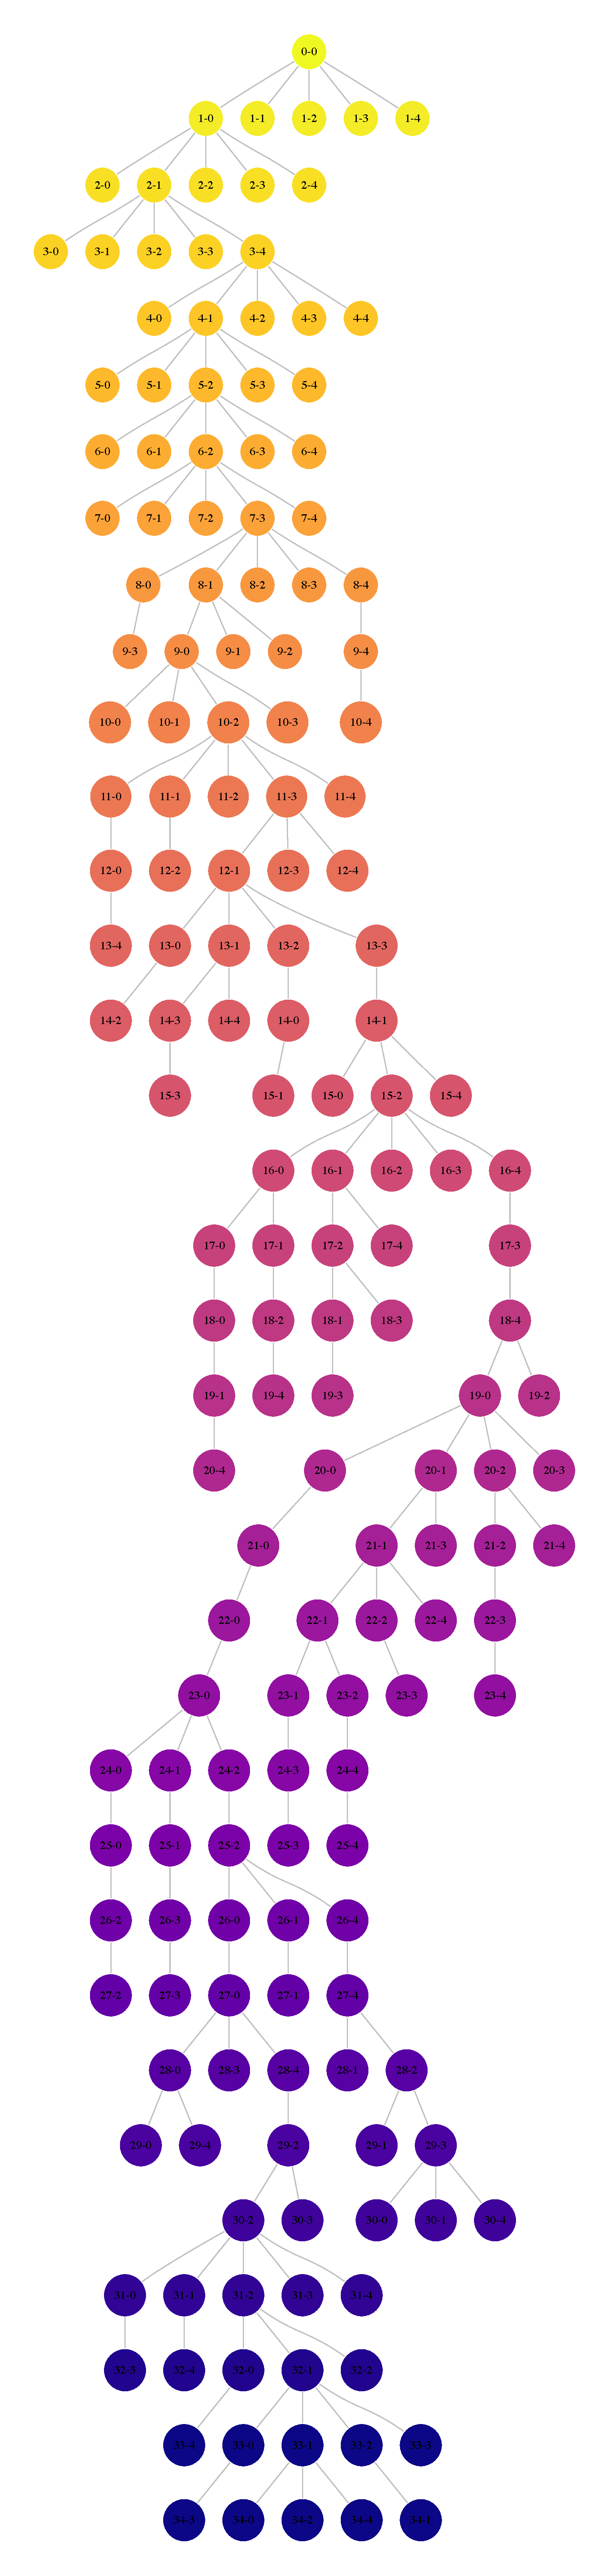
\includegraphics[scale=0.03, angle=90]{Figures/tree_chi_pacs_best.pdf}
 \subcaption{PaCS}
 \end{minipage}
 \begin{minipage}{1.0\hsize}
 \centering
 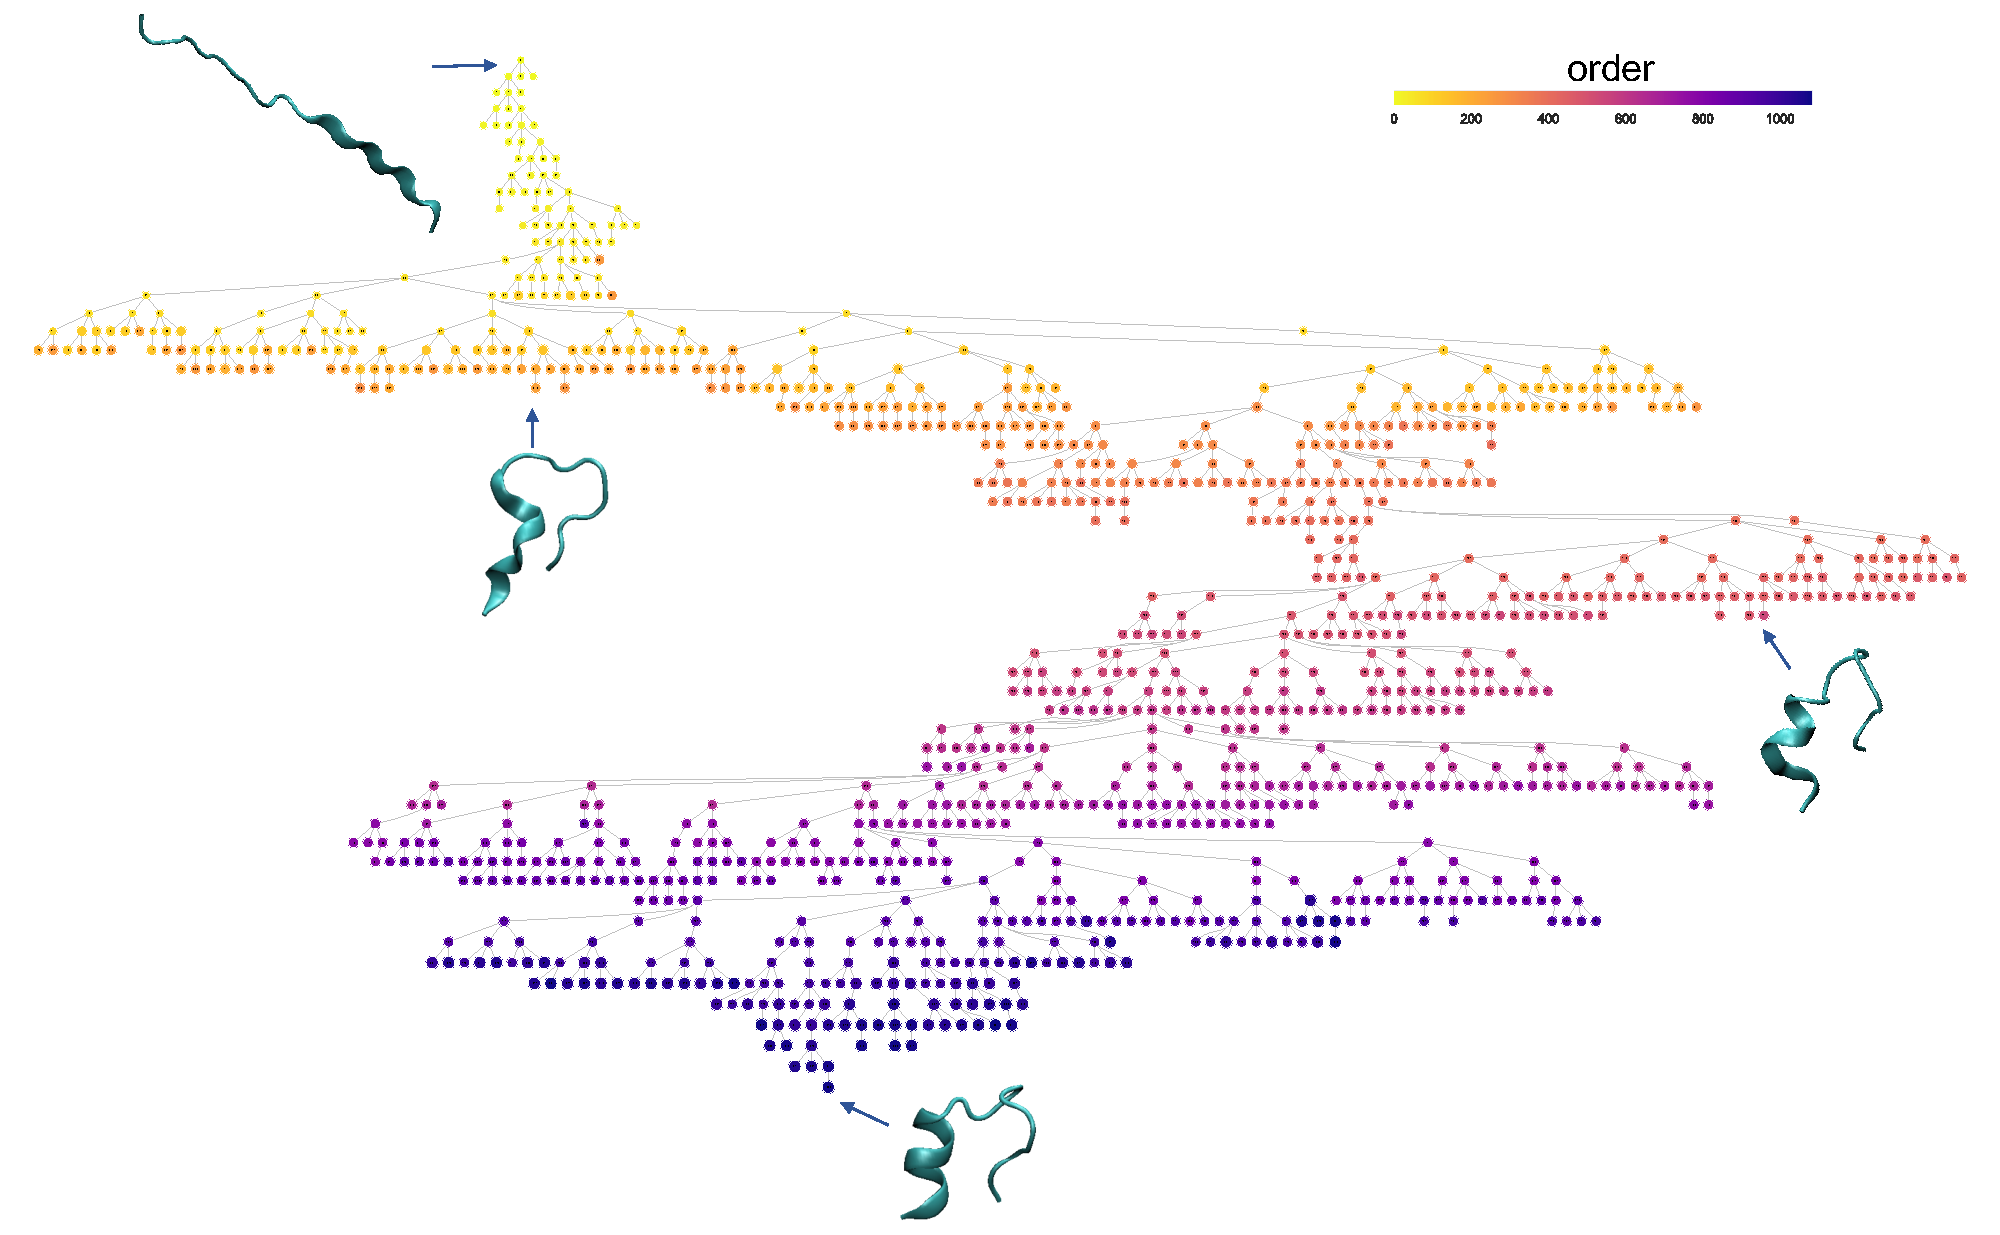
\includegraphics[scale=0.4]{Figures/tree_trp_pats_best.pdf}
 \subcaption{PaTS}
 \end{minipage}
\begin{minipage}{1.0\hsize}
\centering
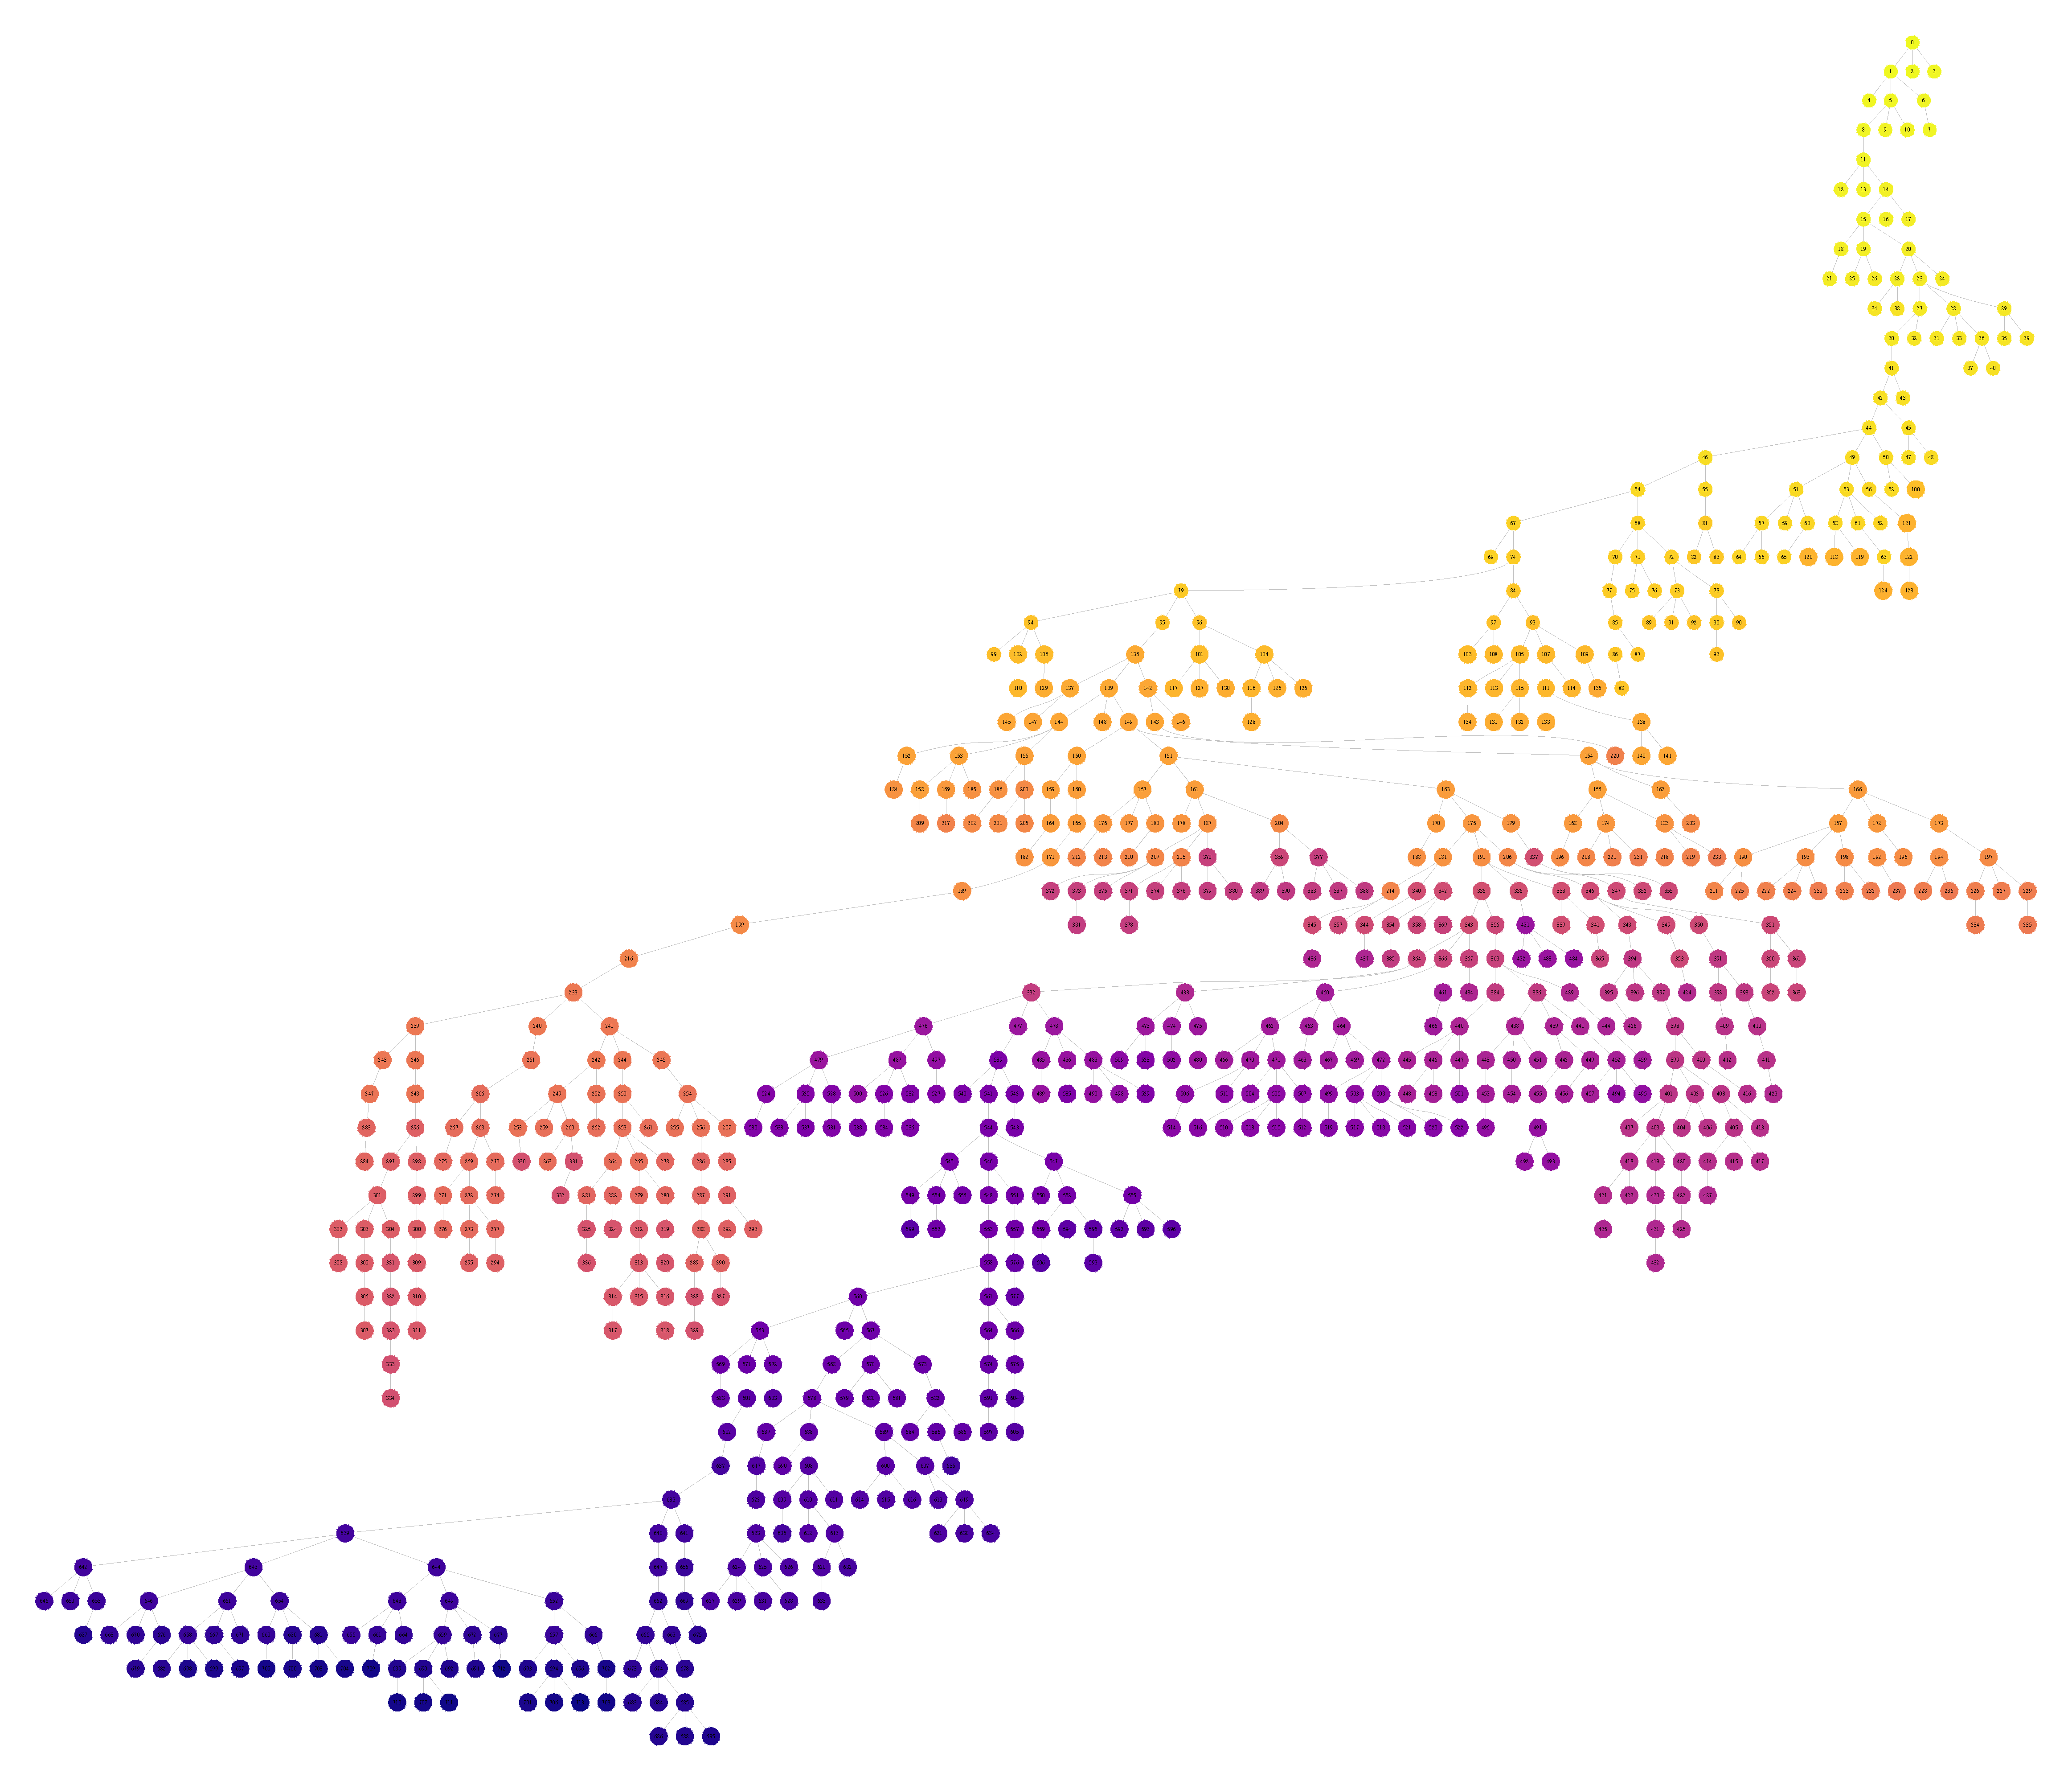
\includegraphics[scale=0.15]{Figures/tree_trp_pats_penal.pdf}
\subcaption{PaTS penalization}
\end{minipage}
\caption{Trees of Trp-cage folding in each methods}
\label{fig:tree_trp}
\end{figure}




\section{Conclusion}
\input{conclusion.tex}

\bibliographystyle{plain}
\bibliography{references}
\end{document}
